% !TEX root = ../main.tex
\newpage
\section{The Theta Neuron Model} \label{TheThetaNeuronModel}
A number of neuron model families have been identified, and often there exists a continuous change of variables from models of the same family into a \textit{canonical} model that can represent the whole family \cite{Hoppensteadt2001CanonicalNM}. As the transformation is not required to be invertible, we can study the universal neurocomputational properties of the family in a low dimensional model.
It was Hodgkin \cite{Hodgkin1948} who classified neurons into two types based on their excitability, upon experimenting with the electrical stimulation of cells. Class 1 models begin to spike at an arbitrarily slow rate, and the spiking frequency increases when the applied current is increased. Class 2 models spike as soon as their internal threshold is exceeded and the spiking frequency stays relatively constant within a certain frequency band \cite{Hoppensteadt2001CanonicalNM}.

\subsection{Model description} \label{sec:TheThetaNeuronModelDescription}

\begin{figure}[H]
\minipage{0.33\linewidth}
\centering
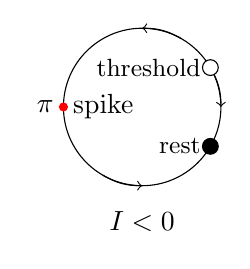
\begin{tikzpicture}
    \draw (0,0) circle [radius=1];
    \draw (0,-1.2) node[below]{$I < 0$};
    \draw (-1,0) node[left]{$\pi$};
    \draw[fill=red, red] (-1,0) circle [radius=0.05];
    \draw (-1,0) node[right]{spike};
    
    \draw[black, ->] (0.866, 0.5)to[out=-60,in=90](1,0);
    \draw[fill=white, draw=black] (0.866,0.5) circle [radius=0.1];
    \draw (0.866,0.5) node[left]{\small{threshold}};
    
    \draw[fill=black, draw=black] (0.866,-0.5) circle [radius=0.1];
    \draw (0.866,-0.5) node[left]{\small{rest}};
    
    \draw[black, ->] (0.5,0.866)to[out=150,in=0](0,1);
    \draw[black, ->] (-0.5,-0.866)to[out=-30,in=180](0,-1);
\end{tikzpicture}
\endminipage
\minipage{0.33\linewidth}
\centering
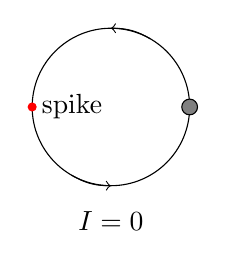
\begin{tikzpicture}
    \draw (0,0) circle [radius=1];
    \draw (0,-1.2) node[below]{$I = 0$};
    \draw[fill=red, red] (-1,0) circle [radius=0.05];
    \draw (-1,0) node[right]{spike};
    
    \draw[fill=gray, draw=black] (1,0) circle [radius=0.1];
    
    \draw[black, ->] (0.5,0.866)to[out=150,in=0](0,1);
    \draw[black, ->] (-0.5,-0.866)to[out=-30,in=180](0,-1);
\end{tikzpicture}
\endminipage
\minipage{0.33\linewidth}
\centering
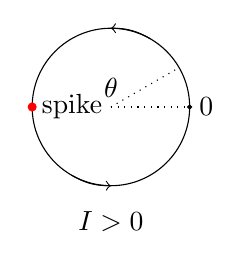
\begin{tikzpicture}
    \draw (0,0) circle [radius=1];
    \draw (0,-1.2) node[below]{$I > 0$};
    \draw (1,0) node[right]{0};
    \draw[fill=black, black] (1,0) circle [radius=0.025];
    \draw[fill=red, red] (-1,0) circle [radius=0.05];
    \draw (-1,0) node[right]{spike};
    
    \draw[black, dotted] (0,0)to(1,0);
    \draw(0,0) node[above]{$\theta$};
    \draw[black, dotted] (0,0)to(0.866,0.5);
    
    \draw[black, ->] (0.5,0.866)to[out=150,in=0](0,1);
    \draw[black, ->] (-0.5,-0.866)to[out=-30,in=180](0,-1);
\end{tikzpicture}
\endminipage
\caption{SNIC bifurcation of the theta neuron model. For $I < 0$, the neuron is in a rest state but excitable. For $I > 0$, the neuron spikes regularly. The bifurcation occurs at $I = 0$. A spike occurs when $\theta = \pi$.}
\label{fig:thetaneuronbifurcationtikz}
\end{figure}

In \cite{Ermentrout1986}, a class 1 canonical phase model was proposed:
\begin{align}
\dot{\theta} = (1-\cos \theta)+(1+\cos \theta) \cdot I \qquad \theta \in \T \label{eq:thetaneuron}
\end{align}
with $I$ a bifurcation parameter on the supplied current. We can visualise the dynamics on the unit circle, like in Figure \ref{fig:thetaneuronbifurcationtikz}. The neuron produces a spike when $\theta$ surpasses $\pi$. As $I$ increases, we see the coalescence of a saddle and node and the neuron starts to fire periodically, we can recognise the features of the class 1 model in Figure \ref{fig:ThetaNeuronResponseToCurrent}. This makes \eqref{eq:thetaneuron} the normal form of the \textit{saddle-node-on-invariant-circle} ($\SNIC$) bifurcation \cite{Luke2013}.

\begin{figure}[H]
\centering
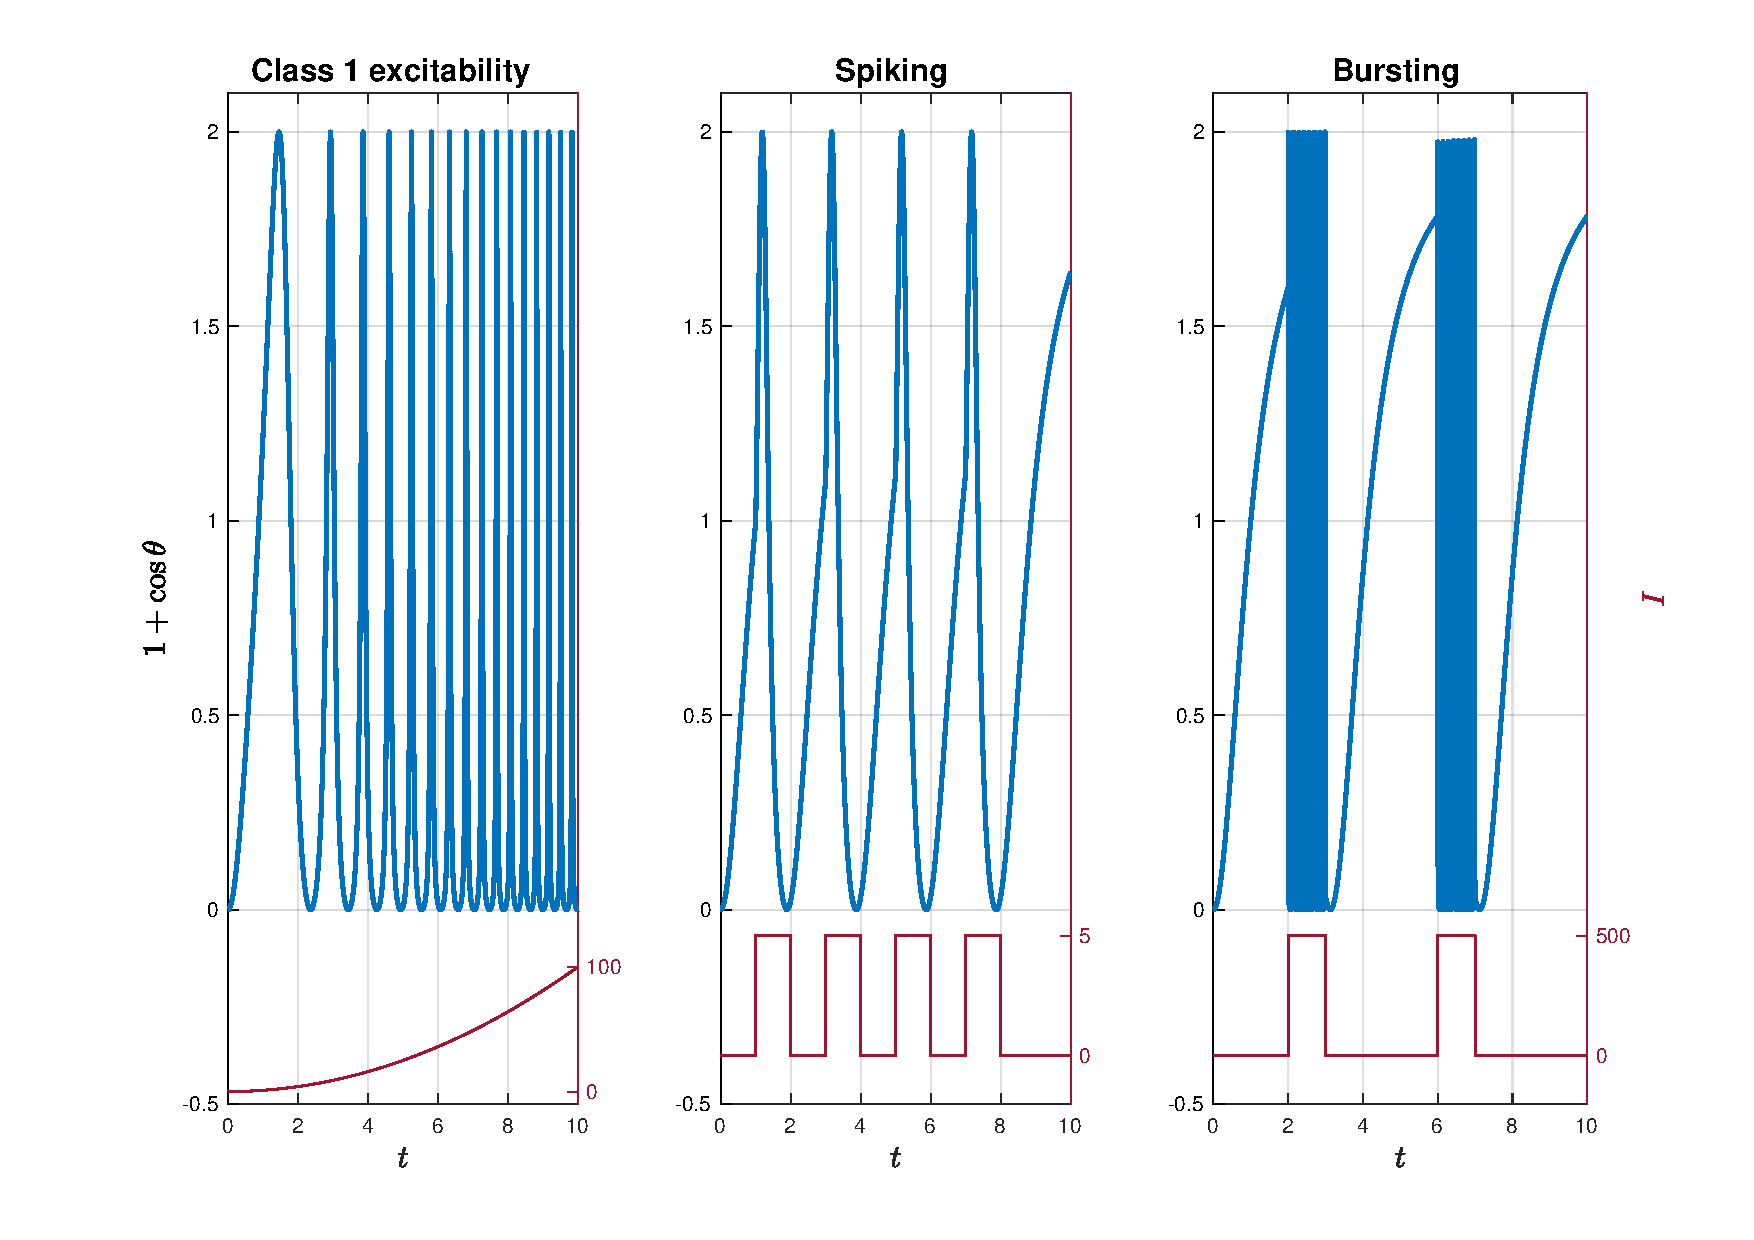
\includegraphics[width = \textwidth]{../Figures/ThetaNeuronResponseToCurrent.pdf}
\caption{Properties of the theta neuron model. Left: the spike frequency of $\theta$ increases as $I$ is increased over time, which is the distinguishing feature of class 1 canonical models. Middle: spikes occur within a finite time period when $I > 0$ and within infite time when $I = 0$. Right: when $I$ is large, the neuron \textsl{bursts}.}
\label{fig:ThetaNeuronResponseToCurrent}
\end{figure}

For $I > 0$, $\dot{\theta} > 0$ so that $\theta$ moves continuously around the circle. Equilibria only exist for $I < 0$: 
\begin{align*}
\dot{\theta} &= 1-\cos \theta+I+I \cdot \cos \theta = (I+1)+(I-1) \cdot \cos \theta \\
\theta^{\ast}_{1, 2} &= \pm \arccos \left(\frac{I+1}{1-I}\right)+2 \pi n
\end{align*}
We can find the stability of the equilibria through:
\begin{align*}
\frac{\mathop{d}}{\mathop{d \theta}}((1-\cos \theta)+(1+\cos \theta) \cdot I) &= \sin \theta-\sin \theta \cdot I = (1-I) \cdot \sin \theta
\end{align*}
In the equilibria this yields:
\begin{align*}
\frac{\mathop{d}}{\mathop{d \theta}}\left( \theta^{\ast}_{1, 2} \right) &= \pm(1-I) \cdot \sqrt{1-\frac{I+1}{1-I}}=\pm(1-I) \cdot \frac{2 \sqrt{-I}}{1-I} = \pm2 \sqrt{-I}
\end{align*}
This yields a stable equilibrium point for $\theta^{\ast}_{1}$ and an unstable for $\theta^{\ast}_{2}$.

\begin{figure}[H]
\centering
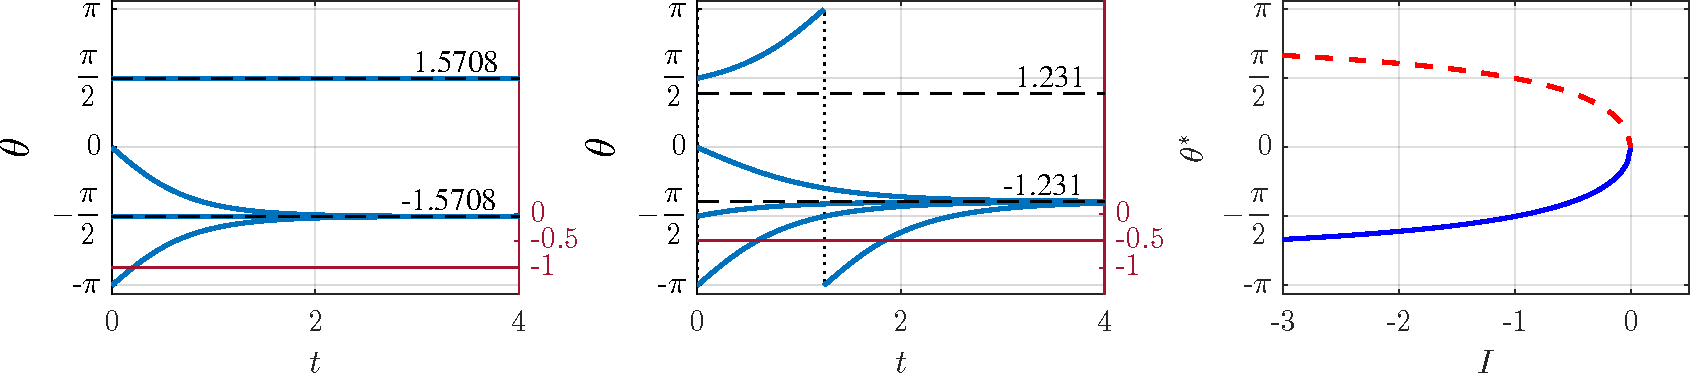
\includegraphics[width = \textwidth]{../Figures/ThetaModelEquilibriumPoints.pdf}
\caption{Equilibria $\theta^{\ast}$ for different values of $I$. Left: $I = -1$ yields $\theta^{\ast} = \pm \frac{\pi}{2}$. Middle: $I = -0.5$. Right: bifurcation diagram of the \SNIC bifurcation, with the stable equilibria in blue, and the unstable in red.}
\label{fig:ThetaModelEquilibriumPoints}
\end{figure}


\subsection{Solutions for static currents} \label{sec:TheThetaNeuronModelSolutions}
Gaining insight into \eqref{eq:thetaneuron} is hard, due to the difficulty of finding an analytical solution. However, it has been noted that there exists a simple transformation which yields (see \ref{app:TransformationToQIF}):
\begin{align}
V &\equiv \tan \left( \frac{\theta}{2} \right) \label{eq:QIFtransformation} \\
\dot{V} &= V^2 + I \label{eq:QIFmodel}
\end{align}
This model is called the \textsl{Quadratic Integrate and Fire model} (\QIF). \eqref{eq:QIFmodel} models the membrane potential of a neuron, which spikes to $=\infty$ when the neuron spikes and is reset at $-\infty$. $V$ and $\theta$ are both continuous on $\T$, so insights from a solution for $V$ can be transformed directly. The solution is (see \ref{app:ThetaModelSolutions}):
\begin{align}
\theta = 2 \cdot \arctan \left(-\sqrt{I} \cdot \cot (t \sqrt{I}) \right) \label{eq:ThetaNeuronModelSolution}
\end{align}


\subsection{Frequency response} \label{sec:TheThetaNeuronModelFrequencyResponse}
As we already saw in Figure \ref{fig:ThetaNeuronResponseToCurrent}, an increasing input current increases the spiking frequency. We can compute this relationship by measuring how long it takes for $V$ to reach a spike: we solve \eqref{eq:ThetaNeuronModelSolution} for $t$ at $V(t) = +\infty$. This tields the oscillation period $T = \frac{\pi}{\sqrt{I}}$. 

\begin{figure}[h]
\centering
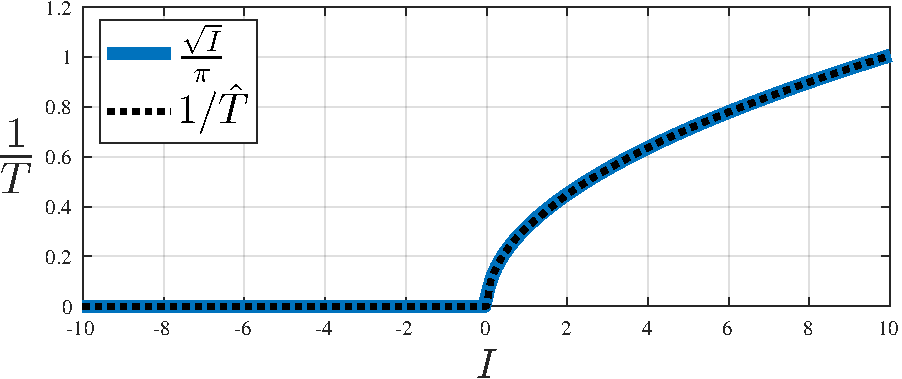
\includegraphics[width = 0.5\textwidth]{../Figures/ThetaNeuronResponseToCurrentPeriod.pdf}
\caption{This is wrong?}
\label{fig:ThetaNeuronResponseToCurrentPeriod}
\end{figure}

In most of our future work, $I$ will not be a static current. We ask ourselves: how much does $T$ change when $I$ is perturbed? We can measure this with the normalised magnitude of the derivative:
\begin{align*}
\left| \frac{dT}{d\iota} \frac{\iota}{T} \right| &= \left| \frac{dT / T}{d\iota / \iota}\right| 
= \left|- \frac{\pi}{2} \left(\frac{1}{\sqrt{\iota}}\right)^3 \frac{\iota}{T} \right| 
= \left| \frac{\pi}{2} \left(\frac{T}{\pi}\right)^3 \frac{\iota}{T} \right| 
= \frac{1}{2} \left|\left(\frac{T}{\pi}\right)^2 \cdot \left(\frac{\pi}{T}\right)^2 \right| = \frac{1}{2}
\end{align*}
Hence, a 1\% change in $I$ will result in a 0.5 \% in $T$


\subsection{Networks of theta neurons}
We can easily extend the model to networks of neurons:
\begin{align}
\dot{\theta}_{i} &=\left(1-\cos \theta_{i}\right)+\left(1+\cos \theta_{i}\right) \cdot \left[\eta_{i} + \kappa \cdot I_{i}(t)\right] \qquad \theta_i \in \T^N  \label{eq:thetaneuronnetwork} \\
I_{i}(t) &=\frac{1}{\kmean} \sum_{j=1}^{N} A_{i j} \cdot \mathcal{P}_{n}(\theta_{j}) \label{eq:thetaneuronnetworkcurrent}
\end{align}
where the excitability is drawn from a distribution and $\mathcal{P}(\theta)  = a_n(1 - \cos \theta)^n$ models synaptic coupling by a pulse-shaped signal, emitted when a neuron fires. $n$ models the sharpness of the pulse, and $a_n$ is a normalisation constant. We will take $n=2$ from here in as in\cite{Luke2013}, \cite{OttAntonsen2017}, \cite{Martens2020}. Another type of coupling is proportional to the difference in voltage between neurons \cite{Martens2020}. Note that for a fully connected network, \eqref{eq:thetaneuronnetworkcurrent} reduces to the scenarios in \cite{Luke2013} and \cite{Martens2020}.


